%amsart class
\documentclass[a4paper, 10pt, reqno]{amsart}

%Packages
\usepackage[utf8]{inputenc}
\usepackage[english]{babel}
\usepackage{graphics}
\usepackage{physics}
\usepackage{listings}
\usepackage[hidelinks]{hyperref}
\usepackage{blindtext}
\usepackage{color}
\usepackage{subfig}
\usepackage{pgf}
\usepackage{tikz}
\usepackage{tikzscale}
\usepackage{pgfplots}
\usepackage{pgfplotstable}
\usepackage{array}

\pgfplotsset{compat=1.5}
%\newlength\figureheight
%\newlength\figurewidth
%\setlength\figurewidth{0.98\textwidth}
%\setlength\figureheight{0.75\figurewidth}


%Custom colors
\definecolor{awesome}{rgb}{1.0, 0.13, 0.32}
\definecolor{royalblue}{RGB}{65, 105, 225}

%Frontpage stuff
\title[The Ising Model]{\Large{Project 4: The Ising Model} \\
\normalsize{FYS4150 - Computational Physics}}

\author[San]{Metin San}

\date{\today}



%Begining document
\begin{document}

\maketitle
\begin{center}
    \textsc{\url{https://github.com/MetinSa/FYS4150/tree/master/Project_4}}
\end{center}

\begin{abstract}
    This project addresses the study of the two-dimensional binary Ising model with focus on phase transitions. We start by studying the expectation values of the $2 \times 2$ square lattice, and gradually work our way up to the $100 \times 100$ lattice. The numerical method used are the Markov Chain based Monte Carlo Metropolis algorithm. By using the critical temperature found in the different simulations we are able to estimate the critical temperature at the thermodynamic limit of $L \rightarrow \infty$ which we find to be $T_C(L = \infty) = 2.2751 J/k_B$ This result is in close accordance with the exact solution derived by Lars Onsager.
\end{abstract}

\section{Introduction}

This project has two primary goals. The first is to study a popular method
of simulating phase transitions, namely the two-dimensional Ising model.
It is a simple and successful model which provides an understanding of
universal critical phenomena which exist in complex materials. We will in
this study consider a ferromagnetic model. Ferromagnetism is a phenomena
where a collection of atomic spins all have their magnetic moments aligned
in the same direction.
The secondary goal is to get familiar with Monte Carlo methods. Monte
Carlo methods are algorithms that uses random sampling as a means to
obtain numerical results. The specific Monte Carlo method of choice during
our study will be the Metropolis algorithm. These methods are highly
applicable in many fields of science, more specifically in statistics and
statistical physics, and is often a saving grace when working with complex
and large systems.

We will start by considering the Ising model with a $2 \times 2$ square
lattice. This is a simple system with known analytic expectation values,
which makes for an a natural and educational start to our studies. After
comparing the extracted expectation values with the analytic ones, we move
on to a $20 \times 20$ lattice. This represents a more complex system
which allows for more detailed and exciting analysis. Finally we will
study even larger systems as a functions of temperature and try to extract
a critical temperature $T_C$ where the system undergoes a phasetransition.

We will begin with a theory section where we cover the physics behind
our study, which is mainly thermodynamics and statistical physics. What
follows is a methods section where we discuss the numerical methods we
have applied in order to simulate the Ising model. We will then present
our results and discuss their credibility and significance. The report is then wrapped up with a conclusion and some final remarks.

The main program is written in \texttt{C++} and the tools used to analyze
the results are in \texttt{python}. All code is located on my Github and can be found by following the URL located beneath the author name on the front page.

\newpage 

\section{Theory}

The Ising model is developed by the German physicist Ernst Ising which studied binary ferromagnetic systems during his doctoral thesis. It quickly became one of the most popular models in the field of statistical physics as a result of its simplicity and success.

\subsection{The Ising Model}We begin by considering a two-dimensional
quadratic lattice. The lattice contains a discrete collection of variables called
spins. This is a binary system where each spin can take on the value $s_k
\pm 1$. In its simplest form, the energy of this model can be expressed as


\begin{equation}\label{eq:energy}
    E = -J \sum_{< kl >}^N s_k s_l,
\end{equation}
where we have assumed that no external magnetic fields are present. Here
$N$ is the total number of spins in the system, and the sum is a double sum
where $<kl>$ means that we sum over the nearest neighbors only. $J$ is a
coupling constant which expresses the strength of the interaction between
neighboring spins and has the units energy. We will assume that $J > 0$ as we are interested in studying a system with ferromagnetic ordering. The magnetic moment or magnetization of the system is simply given as the sum over all spins

\begin{equation}\label{eq:magnetism}
    M = \sum_k^N s_k.
\end{equation}

The system in consideration will be in thermal equilibrium with a constant
temperature. The natural statistical ensemble for such a system is
the canonical ensemble. The configuration probability of a system in the
canonical ensemble is given by the Boltzmann distribution which reads

\begin{equation}\label{eq:boltzmann dist}
    P(i) = \frac{e^{-\beta E_i}}{Z},
\end{equation}
which tells us the probability of the system being in a state $i$ with
energy $E_i$ and temperature $\beta = (k_B T)^{-1}$ where $k_B$ is the
Boltzmann constant. The normalization factor $Z$ is the partition function
which in
the canonical ensemble is given as

\begin{equation}\label{eq:partition func}
    Z = \sum_i e^{-\beta E_i}.
\end{equation}

\subsection{Expectation Values}
We are able to calculate a set of expectation values for a system
described by the above relations. The expectation value of a given
quantity is the average value one expects to find when making a
measurement of said quantity. In general, the expectation value of an
arbitrary quantity $X$ is computed as following

\begin{equation}\label{eq: <X>}
    \langle X \rangle = \sum_i X_i P(i),
\end{equation}
where $X_i$ is the value that $X$ takes on in state $i$, and $P(i)$
is the probability configuration of the model in the same state. The sum is
over all possible configurations, which in out binary model is $2^{L\times L}$
where $L$ is the dimension of the lattice. Using the probability distribution
in equation \eqref{eq:boltzmann dist} we can compute the expectation value of
the energy of the Ising model

\begin{equation}\label{eq: <E>}
    \langle E \rangle = \frac{1}{Z} \sum_i E_i e^{- \beta E_i},
\end{equation}
Similarly the expectation value of the magnetization is given as

\begin{equation}\label{eq: <M>}
    \langle M \rangle = \frac{1}{Z} \sum_i M_i e^{- \beta E_i}.
\end{equation}

Other interesting quantities are for instance the heat capacity $C_V$ also
known as the specific heat which is the amount of thermal energy (heat)
required to change the temperature of the system. This is a measurable
quantity, and its expectation value is given as

\begin{equation}\label{eq: C_V}
    C _ { V } = \frac { 1 } { k _ { B } T ^ { 2 } } \left( \langle E^2 \rangle - \langle E \rangle^2 \right).
\end{equation}
Another quantity that we will study is the magnetic susceptibility $\chi$
which is a dimensionless proportionality constant. It indicates the degree of
magnetization in our system and is given as

\begin{equation}\label{eq: chi}
    \chi = \frac { 1 } { k _ { B } T } \left( \langle M^2 \rangle - \langle M \rangle^2 \right).
\end{equation}
The terms appearing in the numerators of equations \eqref{eq: C_V} and
\eqref{eq: chi} are the respective variance of the energy and magnetism. The
variance is an important statistical quantity and describes the squared
deviation of a variable from its mean. In general, the variance of an
arbritary quantity $X$ is given as

\begin{equation}\label{eq: var}
    \sigma^2_X = \langle X^2 \rangle - \langle X \rangle ^2,
\end{equation}
where $\sigma_X$ is the standard deviation of $X$. We note that computing the
different expectation values allow us to study the statistical features of
the system.

\subsection{Unit Scaling} It is often wise to rescale and tailor certain
quantities to the specific system one studies. Scaling units allows us to
work in a more controlled and usually a more intuitive size scale. Perhaps
the most important consequence of scaling is that it often generalizes the
mathematical expressions one works with which in turn can make the underlying
physics more transparent.

During our study, we will scale the temperature $T$ by multiplying it with
the Boltzmann constant $k_B$ divided by the coupling constant $J$, so that
the new temperature is $T' = T k_B/J$. This appears to be a natural
rescaling for our Ising model as it allows us to ignore the constants $k_B$
and $J$ throughout the analysis. It also turns the temperature $T'$ into a
dimensionless quantity. We will also refer to the critical temperature $T'_C k_B /J$ as simply $T_C$ through out this study.


\subsection{The $2\times 2$ Lattice} There is always the
possibility that the results one obtain through numerical methods are
affected by errors with the implementation of said method. Having analytical
results which can be used for comparison is therefore invaluable. We will
therefore begin the analysis by deriving the analytical results for the
simple $2 \times 2$ spin lattice. This will give some initial intuition into
the behaviour of the model and the results will be used to test the
functionality of our code.

\begin{figure}[h]
	\centering
	\subfloat[]{
	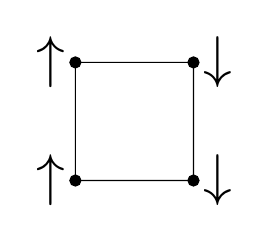
\begin{tikzpicture}
	\filldraw 	(0,0) circle(2pt) node[align=left, left]{\huge{$\uparrow$}}-- 
				(0,1.5) circle(2pt) node[align=left, left]{\huge{$\uparrow$}}-- 
				(1.5,1.5) circle(2pt) node[align=right, right]{\huge{$\downarrow$}}-- 
				(1.5,0) circle(2pt) node[align=right, right]{\huge{$\downarrow$}}-- (0,0);
	\end{tikzpicture}} \hspace{10mm}
	\subfloat[]{
		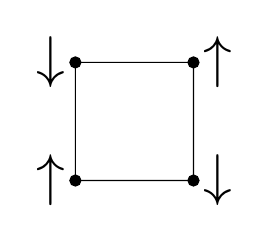
\begin{tikzpicture}
	\filldraw 	(0,0) circle(2pt) node[align=left, left]{\huge{$\uparrow$}}-- 
				(0,1.5) circle(2pt) node[align=left, left]{\huge{$\downarrow$}}-- 
				(1.5,1.5) circle(2pt) node[align=right, right]{\huge{$\uparrow$}}-- 
				(1.5,0) circle(2pt) node[align=right, right]{\huge{$\downarrow$}}-- (0,0);
	\end{tikzpicture}}
	\caption{ The doublet state of the $2\times2$ spin lattice. Both
	microstates have 2 spins up and 2 spins down. The associated energy and
	magnetization of configuration (A) is $E_{(A)} = 0$ and $M_{(A)} = 0$
	respectively, while the energy and magnetization of configuration (B) is
	$E_{(B)} = 8J$ and $M_{(B)} = 0$.}
	\label{fig: 2x2}
\end{figure}

\begin{table}
\caption{All possible microstates and their corresponding degeneracy, energy and magnetization in the Ising model for a $2 \times 2$ lattice.  }
\label{tab: 2x2}
\begin{tabular}{llrr}
\hline
Number of spins up & Degeneracy & Energy $(E)$ & Magnetization $(M)$ \\ \hline
0 & 1 & -8J & -4 \\
1 & 4 & 0 & -2 \\
2 & 2 & 8J & 0 \\
2 & 4 & 0 & 0 \\
3 & 4 & 0 & 2 \\
4 & 1 & -8J & 4 \\ \hline
\end{tabular}
\end{table}

\subsubsection{Analysing the microstates} For a $L = 2$ lattice, we have $2^{2\times 2} = 16$ different
configurations (microstates). For such a small system one can easily draw and
study every configuration individually. By using equations \eqref{eq:energy}
and \eqref{eq:magnetism}, we are able to compute the energy and magnetization
for each state respectively. We find that there are 2 configurations where
all the spins point in the same direction which results in an energy of $E_i
= -8J$ and $M_i = \pm 4$ depending on the orientation of the spins. There are
8 different configurations where the system has three parallel and one
anti-parallel spin, all with the energy $E_i = 0$ as and $M_i =  \pm 2$. We
find 4 different configurations with 2 parallel and 2 anti-parallel spins
which yield the energy $E_i = 0$ and the magnetism $M_i =0$. However, there
are 2 additional configurations which also have two spins up and two down,
where the energy instead sums to $E_i = 8J$ and $M_i = 0$, meaning that the
configuration of 2 spin up and 2 down is a doublet state. The doublet state is shown in more detail in figure \ref{fig: 2x2}. This concludes all
the microstates. The results have been tabulated in table
\ref{tab: 2x2}.

\subsubsection{Expectation Values} We will now continue by computing the
expectation values for the $2\times 2$
system. In order to do so we need to compute the partition function $Z$ seen
in equation \eqref{eq:partition func}. The calculation results in

\begin{equation*}
    Z  = 2 e^{ 8\beta J} + 2e^{-8 \beta J} + 12,
\end{equation*}
where we have inserted all the non zero energy states. This can be
rewritten in terms of the hyperbolic function $\cosh(x) = (\exp(x) +
\exp(-x))/2$. We will also put the unit scaling discussed in the above
section into use so that the final partition function in the $2 \times 2$
system reads

\begin{equation}\label{eq 2x2 part}
    Z = 4 \cosh (8/T') + 12,
\end{equation}
where $\beta$ has been written out in terms of $T' = k_BT/J$. With the partition function in place, we can move on to
compute the various expectation values. The expectation values of the energy
is found following equation \eqref{eq: <E>} which gives us

\begin{equation}\label{eq: 2x2 <E>}
    \langle E \rangle = \frac{1}{Z} \left(-16J e^{8/T'} + 16J e^{-8/T'}\right) = \frac{-8J \sinh(8/T')}{\cosh(8/T') + 3},
\end{equation}
where we have used the hyperbolic function $\sinh(x) = (\exp(x) -
\exp(-x))/2$.

We find the other expectation values by similar calculations, starting with
the energy squared which is given as

\begin{equation}\label{eq: 2x2 <E^2>}
    \langle E^2 \rangle = \frac{1}{Z}\left[ (-16J)^2 e^{8/T'} + (16J)^2 e^{-8/T'}\right]= \frac{64 J^2 \cosh (8/T')}{\cosh(8/T') + 3}.
\end{equation}
The expectation value of the magnetization is 0 as seen below

\begin{equation}\label{eq: 2x2 <M>}
    \langle M \rangle = \frac{1}{Z} \left(-4e^{8/T'} - 8 + 8 + 4e^{8/T'}\right) = 0.
\end{equation}
A more interesting quantity is therefore the absolute value of the magnetization which is given as

\begin{equation}\label{eq: 2x2 <absM>}
    \langle \abs{M} \rangle = \frac{1}{Z} \left(4e^{8/T'} + 8 + 8 + 4e^{8/T'}\right) = \frac{2e^{8/T'} + 4}{\cosh(8/T') +3}.
\end{equation}
The magnetization squared is given as

\begin{equation}\label{eq: 2x2 M^2}
    \langle {M}^2 \rangle = \frac{1}{Z}\left( 32e^{8/T'} +32 \right) = \frac{8e^{8/T'} + 8}{\cosh(8/T') +3}.
\end{equation}
The heat capacity $C_V$ is easy to derive as we already have both the
expectation value of the energy and its squared from equations \eqref{eq: 2x2
<E>} and \eqref{eq: 2x2 <E^2>}. By substituting these into the expression for the specific heat in \eqref{eq: C_V} we find the following 

\begin{align}
    C_V =& \frac{1}{k_B T^2} \left( \frac{64J^2 \cosh(8/T')}{\cosh(8/T') +3} -
    \frac{64J^2 \sinh^2(8/T')}{(\cosh(8/T') + 3)^2}  \right) \\
    =&\frac{64J^2}{k_B T^2} \left( \frac{\cosh(8/T')(\cosh(8/T') + 3) -
    \sinh^2(8/T')}{(\cosh(8/T') + 3)^2} \right).
\end{align}
We can further use the trigonometric identity $\cosh^2(x) - \sinh^2(x) = 1$ to reduce the above expression to the final form

\begin{equation}\label{eq: 2x2 C_V}
  C_V  = \frac{64k_B}{T'^2}\left( \frac{1 + 3\cosh(8/T')}{(\cosh(8/T') + 3)^2} \right),
\end{equation}
where we have also rewritten $T$ in terms of the scaled temperature.
The susceptibility is computed in a similar way. We know that the expectation value of the magnetization is 0, so the expression is simplified to

\begin{equation}\label{eq: 2x2 chi}
    \chi = \frac { 1 } { k _ { B } T }\langle M^2 \rangle = \frac{8}{k_B T} \left(\frac{e^{8/T'} + 1}{\cosh(8/T') +3}\right) = \frac { 8 }{JT'} \left( \frac{e^{8/T'}+1}{\cosh(8/T') + 3} \right)
\end{equation}

It should be noted that some of the above equations could have been more easily derived using known expressions from thermal physics. We have done it this way to show the power of statistical physics, where we are able to derive several desired quantities by simply having the expectation values.

\subsection{Phase Transitions and The Critical Temperature}
A magnetic system is said to have undergone a phase transition if it moves from a magnetic phase to a phase with no magnetization. The temperature at which this transition occurs is the so called critical temperature $T_C$. When a system is near the critical temperature many of the physical quantities associated with the system can be described by power laws. In the Ising model, the mean magnetization is given by 

\begin{equation} \label{eq: T_C <M>}
    \langle M (T) \rangle \sim (T - T_C)^\beta.
\end{equation}
Similarly, the heat capacity and susceptibility is given as

\begin{equation} \label{eq: T_C <C_V>}
    C_V(T) \sim \abs{T_C - T}^\alpha
\end{equation}
\begin{equation} \label{eq: T_C <chi>}
    \chi(T) \sim \abs{T_C - T}^\gamma.
\end{equation}
The exponents $\alpha$, $\beta$ and $\gamma$ are the so-called critical exponents, and they have the following values $\alpha = 0$, $\beta = 1/8$, $\gamma = 7/4$.

Another important quantity in the Ising model is the correlation length $\xi$ which is expected to be of the same order as the lattice spacing when temperatures are much greater than the critical temperature. The spins should get more and more correlated as the temperature approaches the critical temperature, meaning that the correlation length will increase as we get closer to the $T_C$. The divergent behaviour of the correlation length near the critical temperature also resembles a power law and is given as

\begin{equation}\label{eq: xi}
    \xi(T) \sim \abs{T_C - T}^\nu.
\end{equation}
The phase transition which occurs at the critical temperature is characterized by a correlation length which spans the entire system. We are however always limited to finite lattices, so we take the correlation length $\xi$ to be proportional to the size of the lattice. We can then through so-called finite size scaling relations relate the behaviour of our finite lattice to those of infinitely large lattices. Using these relations, we find the critical temperature to scale as

\begin{equation}\label{eq: T_C scale}
    T_C(L) - T_C(L = \infty) = aL^{-1/\nu},
\end{equation}
where $a$ is a constant and $\nu$ is defined in equation \eqref{eq: xi}. The above relation can then be solved for the critical temperature in the thermodynamic limit of $L \rightarrow \infty$

\begin{equation}\label{eq: T_C}
    T_C(L=\infty) =T_C(L) - aL^{-1/\nu}.
\end{equation}
The exact critical temperature for the Ising model was derived by Lars Onsager in 1944 and was found to be

\begin{equation}
    T_C = \frac{2}{\ln(1 + \sqrt{2})}\frac{J}{k_B} \approx 2.269\frac{J}{k_B}
\end{equation}.

The constant $a$ in equation \eqref{eq: T_C} can be found by comparing two different lattice sizes. We can write the following

\begin{equation}
    \left( T_C(L_1) - T_C(L = \infty) \right)-\left( T_C(L_2) - T_C(L = \infty) \right) = a(L_1^{-1/\nu} - L_2^{-1/\nu}),
\end{equation}
which can then be solved for $a$

\begin{equation}\label{eq: a}
    a = \frac{T_C(L_1) - T_C(L_2)}{L_1^{-1/\nu} - L_2^{-1/\nu}}.
\end{equation}
This assumes that we have computed the critical temperature for the respective lattice sizes $L_1$ and $L_2$. The method we will use to find $T_C(L)$ will be to extract the temperature where the heat capacity and susceptibility are at a maximum. We will use $\nu = 1$ through out our studies.

\section{Method}
In this section we will discuss the various numerical methods and technicalities used for the Ising model. The choice of which numerical method one wants to implement during a study is naturally governed by the physics of the problem at hand. For the Ising model a natural choice is the Monte Carlo Metropolis scheme. This is because the evolution of the Ising model can be viewed as a set of Markov processes, which makes up base of Monte Carlo methods. We will begin this section by elaborate on the Monte Carlo Metropolis algorithm, starting with a brief introduction to Markov chains.

\subsection{Markov Chains and Monte Carlo Methods}
A Markov Chain is a stochastic model and can be thought of as a random process or a walk with a selected transition probability. Markov chains are commonly used in physics, for instance when one describes diffusion or Brownian motion, but it also applicable to the Ising model. A feature of the Markov chain is that the system eventually reaches the most likely state if given enough time. This means that a thermodynamic system such as our Ising model will after a certain number of Markov processes reach an equilibrium distribution, which is in accordance with our intuitive understanding of the world. Monte Carlo methods are a broad class of algorithms based on random sampling, some of which are Markov chain Monte Carlo methods which makes use of the above discussed features of the Markov Chains. The Monte Carlo method which we will use in this study is the Metropolis algorithm.

\subsection{The Metropolis algorithm}
In order to reach this equilibrium, the Markov process need to follow two conditions, namely ergodicity and detailed balance. Ergodicity means that all microstates of a system is equally probable over if given long enough time. Detailed balance means that in equilibrium, a process can be equilibrated by its inverse process. This can be formulated mathematically to read

\begin{equation}\label{eq: mark}
    W_{i \rightarrow j}w_i = W_{j \rightarrow i }w_j,
\end{equation}
where $w_i$ is the probability distribution for state $i$ which in the Ising model is given through the Boltzmann distribution from equation \eqref{eq:boltzmann dist}. $W_{i \rightarrow j}$ is the total transition probability of going from state $i$ to $j$ and is given as
\begin{equation}
    W_{i \rightarrow j} = T_{i \rightarrow j} A_{i \rightarrow j},
\end{equation} 
where $T_{i \rightarrow j}$ is the probability of trying a transition, and $A_{i \rightarrow j}$ is the probability of this transition being accepted. Inserting for $w_i$, the transition probability for the Ising model reads

\begin{equation}
    T_{i \rightarrow j} A_{i \rightarrow j} = \frac{1}{Z}e^{-\beta E_i}.
\end{equation}
The partition function $Z$ can be near impossible to calculate, especially for large systems. However, by looking at the ratio between two transition probilities
\begin{equation}\label{eq: mark ratio}
    \frac{ W_{i \rightarrow j}}{ W_{j \rightarrow i}}= \frac{T_{i \rightarrow j} A_{i \rightarrow j}}{ T_{j \rightarrow i} A_{j \rightarrow i}} = \frac{w_j}{w_i} = e^{-\beta\Delta E},
\end{equation}
where $\Delta E = E_j-E_i$, we see that this nasty beast cancels. We will further assume that the transition probability is symmetric so that $T_{i \rightarrow j} = T_{j \rightarrow i}$, meaning that the acceptance probability is simply

\begin{equation}
    \frac{A_{i \rightarrow j}}{A_{j \rightarrow i}} = e^{-\beta\Delta E}.
\end{equation}
Since we are interested in accepting as many moves as possible in order to increase the efficiency of our program, we set the the acceptance probability ${A_{j \rightarrow i}} = 1$. The probability of accepting a move is then given as

\begin{equation} \label{eq: A prob}
   A_{i \rightarrow j} =  e^{-\beta\Delta E}.
\end{equation}
When implementing this method in our code, we simply generate a random number $r$ and compare it to the acceptance probability. If $A_{i \rightarrow j} \geq r$ we accept the move. This condition impose a constraint on our algorithm for when a move can be accepted or must be rejected and is called the Metropolis algorithm.

\subsection{Periodic Boundary Conditions} The lattice we will be working with
is a quadratic two-dimensional $L \times L$ spin lattice. We note that the
spins located at the boundaries of the lattice will have less neighboring
spins than the more centralized spins. This is problematic as the interaction
between neighboring spins are essential to our model.

We solve this problem by introducing Periodic Boundary Conditions (PBCs)
which is a set of boundary conditions often used when one needs to simulate
large systems. One can understand PBCs by imagining that objects moving
through one side of the lattice re-appears on the opposite side. This
condition will allow any boundary spin on the lattice to interact with its
opposite boundary counterpart.

\subsection{Random Number Generators}

The use of a proper Random Number Generator (RNG) is imporant when one works with Monte Carlo simulations. Our method requires the sampling of billions of uncorrelated random numbers. Most standard RNGs have periods of $10^9$. This might be plenty for most common uses, but when one needs to do extensive Monte Carlo simulations this period is often exceeded. What happens then is that the statistical features are produced by correlated random numbers leading to false results. It is therefore of importance to choose a RNG with a period that will not be surpassed. For this purpose, we use the Merseene twister RNG which has a period $2^{19937}$.


\subsection{Implementing the methods}
Here follows an overview of the programs used to solve the Ising model. The main program is written in \texttt{c++} and is found in the \textbf{src} folder. The code is written using an object-oriented approach. The main program consists of the \texttt{Ising} class which contains all the methods necessary to simulate the model, with the most important ones being the \texttt{InitializeLattice}, \texttt{getEnergy} ,\texttt{Metropolis} and \texttt{MonteCarloSample} functions. The method names speak for them selves, but here follows a little overview of their functionality.

\begin{description}
    \item[\texttt{InitializeLattice}] Generates the initial state of our lattice for a given $L$ and $T'$. It also computes the initial energy and magnetization of the lattice and initializes the RNG of choice.  
    \item[\texttt{getEnergy}] Computes $\Delta E$ for a spin and its neighbors a given lattice point, making use of the PBC.
    \item[\texttt{Metropolis}] For a move, compares a random number $r$ generated by the RNG to $\Delta E$ and decides whether or not the move should be accepted. If the move is accepted, the spins in the lattice are flipped.
    \item[\texttt{MonteCarloSample}] Function that binds the other methods together. Executes the Metroplolis algorithm for a given number of Monte Carlo cycles (MC) and updates the expectation values of interest.
\end{description}
In addition to the \texttt{c++} program, we have included a asortment of different tools written in \texttt{python}. These tools can be found in the \textbf{tools} folder and are used to process the data and produce the following figures seen in the Results / Discussion section.

\subsection{Optimizing computing time}
Working with large lattices and many MC cycles, takes its toll on the average computer. We have therefore written a parallel code which is seen in the \texttt{main.cpp} file, where we have used MPI (Message Passing Interface). This parallelizing is specifically meant for the calculations considering "continuous" temperature ranges, but is tailored to also work for single temperature cases. MPI allows us to distribute the temperature array to different processes so that multiple CPU's can work simultaneously to shorten the computational time.  

Another trick which has been implemented is to precalculate the energies. Because of the simplicity of the Ising model, the different available energies are finite and quantized, meaning that we can precompute them to speed up the calculations.

\subsubsection{Computer specifics}
The results used in this study has been computed at the computer cluster "Beehive" through the Institute of Theoretical Astrophysics, which allowed for very fast calculations. Specifically, Beehive20 was used which has 40 CPU's. The calculation times ranged from 6 minutes to 1 and a half hours depending on the lattice size and choice of MC cycles.

\section{Results / Discussion}

We will now present the the different simulations done during the study, the results obtained from these and also provide some discussion around the results.

\subsection{The $2 \times 2$ Lattice} As mentioned in the theory section, we  start by testing the method for the simple $L = 2$ case in order to make sure that the code is functioning as desired. We start by computing the analytic values seen in equations \eqref{eq: 2x2 <E>}, \eqref{eq: 2x2 <M>}, \eqref{eq: 2x2 <absM>}, \eqref{eq: 2x2 C_V} and \eqref{eq: 2x2 chi} using a temperature of $T' = 1$. We then perform Monte Carlo simulations for 6 log-distributed MC cycles $\in [10,10^6]$. For each number of MC cyles we run 100 simulations and average the resulting expectation values. The results of this calculation are tabulated in table \ref{table: 2x2}. 

We observe the desired results where the numerically computed expectation values approach the analytic ones with increasing number of MC cycles. These results suggests that the program is operating as desired, and we can now move on to more complex and interesting models.

\begin{table}[]
\begin{tabular}{llllll}
\hline
MC cycles & $\langle E \rangle$ & $\langle M \rangle$ & $\langle \abs{M}\rangle$ & $C_V$ & $\chi$ \\ \hline
$10$ & $-1.85200$ &-0.40050  & 0.95250 & 0.85440 & 0.24030 \\
$10^2$ & $-1.97400$ & 0.13290 & 0.99090 &0.19990 & 0.21101 \\
$10^3$ & $-1.99452$ & -0.02594 & 0.99816 & 0.04360 & 0.97093 \\
$10^4$ & $-1.99630$ & 0.00461 & 0.99878 & 0.02947 & 3.09485 \\
$10^5$ & $-1.99594$ &0.00369&  0.99865 &0.03233 & 3.90673 \\
$10^6$ & $-1.99595$ & -0.00800 & 0.99865 & 0.03227 & 3.98651 \\ \hline
Analytical & -1.99598 & 0 & 0.99866 & 0.03208 &3.99330\\ \hline
\end{tabular}
\caption{Comparison between the numerically computed and analytic expectation values for the $2 \times 2$ lattice.}
\label{table: 2x2}
\end{table}

\subsection{The $20 \times 20$ Lattice} The $L=20$ lattice is a mouthful analytically but proves to be no match for our numerical model. We will use this lattice size to study how the expectation values evolve with increasing numbers of MC cycles. We start by considering the lattice in an initial configuration with the spins aligned randomly. Simulating the system in consideration for a total of $10^6$ MC cycles gives us a good understanding of how the expectation values evolve.

\begin{figure}
    \centering
    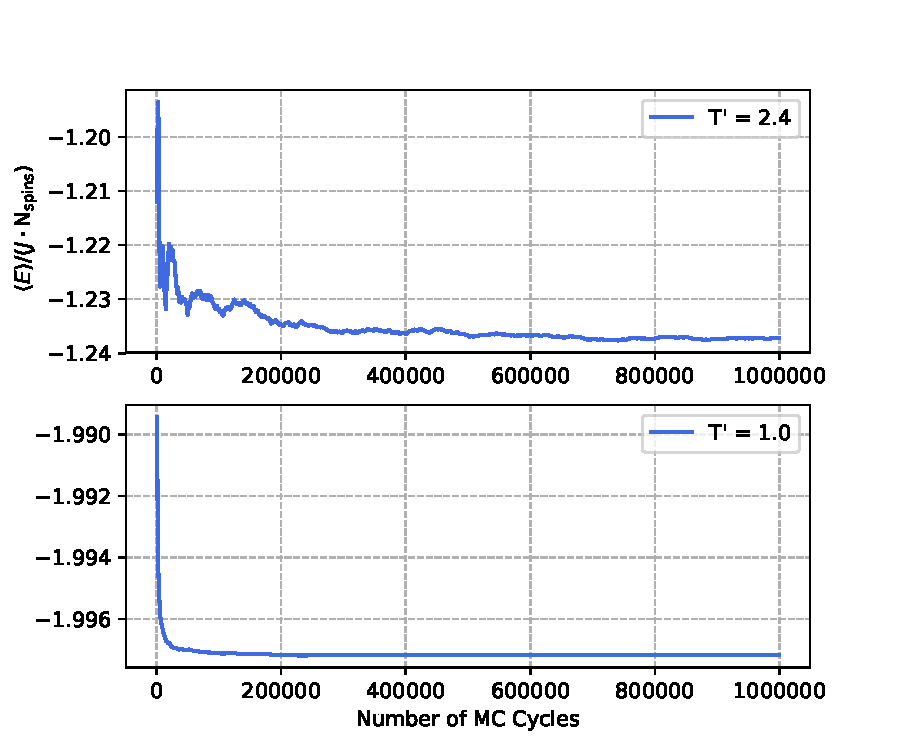
\includegraphics[width=0.95\textwidth]{figures/randomE.pdf}
    \caption{The energy expectation value as a function of MC cycles for a random initial lattice configuration. The lower subplot shows the evolution for a lattice at temperature $T'=1$ and the upper subplot for $T'=2.4$.}
    \label{fig: 20x20 random <E> }
\end{figure}

\begin{figure}
    \centering
    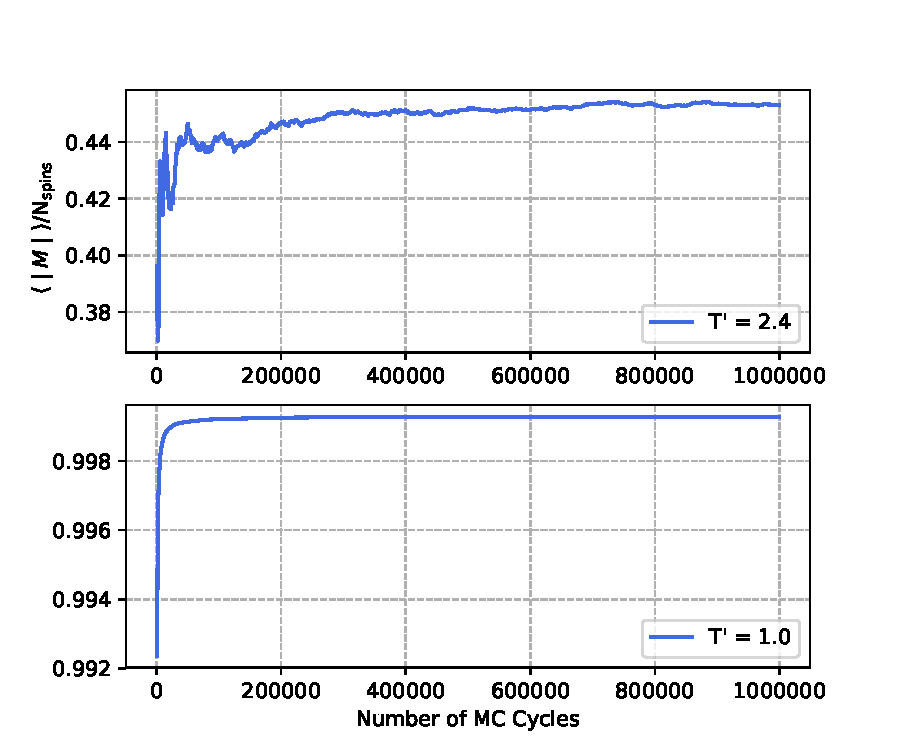
\includegraphics[width=0.95\textwidth]{figures/randomabsM.pdf}
    \caption{The magnetization expectation value as a function of MC cycles for an random initial lattice configuration. The lower subplot shows the evolution for a lattice at temperature $T'=1$ and the upper subplot for $T'=2.4$.}
    \label{fig: 20x20 random <absM> }
\end{figure}

\subsubsection{Energy and Magnetization Expectation Values} By extracting the different expectation values every $10^3$ cycle we are able to produce the results seen in figures \ref{fig: 20x20 random <E> } and \ref{fig: 20x20 random <absM> }. The simulations seen in these figures display the behaviour of the energy and absolute magnetization for two different temperatures $T'=1$ and $T'=2.4$. We notice that both the energy and magnetization with $T' = 1$ quickly converges towards a final expectation value already at sub 50000 MC cycles. The two simulations with $T' = 2.4$ however experiences a more spiky beginning, and we observe the more "common" Monte Carlo behaviour. These observed oscillating features occur as a result of the fact that the system has to evolve for a while before it reaches equilibrium. The expectation values continue to oscillate after equilibrium has been reached but at a much smaller magnitude, slowly creeping closer to the their true value.

\begin{figure}
    \centering
    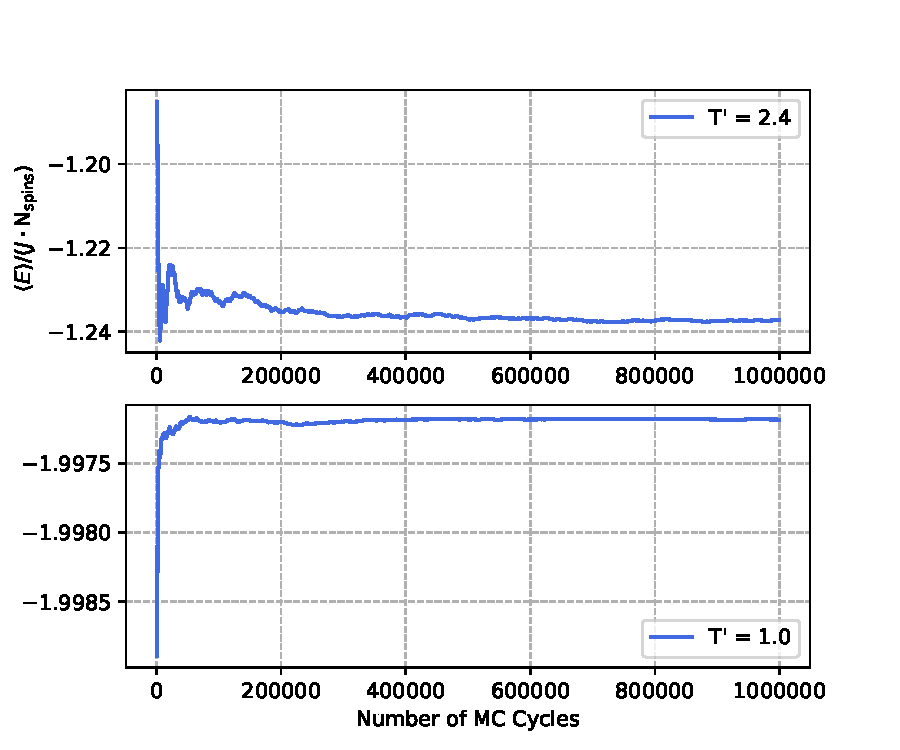
\includegraphics[width=0.95\textwidth]{figures/orientedE.pdf}
    \caption{The energy expectation value as a function of MC cycles for an ordered initial lattice configuration. The lower subplot shows the evolution for a lattice at temperature $T'=1$ and the upper subplot for $T'=2.4$.}
    \label{fig: 20x20 ordered <E> }
\end{figure}

\begin{figure}
    \centering
    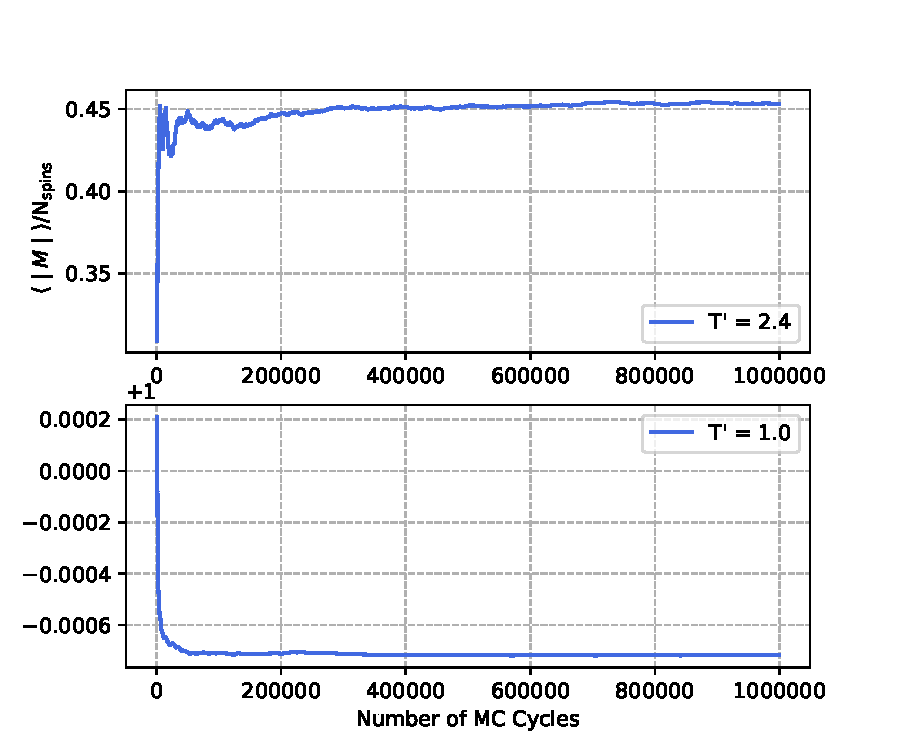
\includegraphics[width=0.95\textwidth]{figures/orientedabsM.pdf}
    \caption{The magnetization expectation value as a function of MC cycles for an ordered initial lattice configuration. The lower subplot shows the evolution for a lattice at temperature $T'=1$ and the upper subplot for $T'=2.4$.}
    \label{fig: 20x20 ordered <absM> }
\end{figure}

We can also look at another scenario where the system now starts of with an ordered initial configuration meaning that we align all the spins. Similarly to the random oriented scenario, we simulate the $L=20$ lattice for the two temperatures $T' = 1$ and $T' = 2.4$. The results can be seen in figures \ref{fig: 20x20 ordered <E> } and \ref{fig: 20x20 ordered <absM> }. By studying these figures we see that the $T' = 2.4$ simulation behaves similar to the case of the random configuration. However, the $T' = 1$ case displays a noticeable difference. We observe that the absolute magnetization barely changes. This is likely because at lower temperatures, the spins are naturally very aligned, meaning that the magnetization was nearly in equilibrium from to begin with. This suggests that the ordered initial configuration is a better approximation to the true system for lower temperatures.
Despite the different initial configurations, both expectation values converge towards the same value with increasing MC cycles. 

\subsubsection{Determining Equilibrium}
The concept of equilibrium plays an important role in MC simulations. The expectation values computed prior to the system having reached an equilibrium state are not accurate and should normally not be considered as representative values. Different initial conditions results in different equilibrium times as observed in the previously discussed figures. For instance, we see that in figure \ref{fig: 20x20 random <E> }, the system with $T' =1$ stabilized a lot faster than the system with $T' = 1$. It it therefore of importance to determine at which MC cycle the system reaches equilibrium. There are many methods of estimating this time,some which are listed below.

\begin{description}
    \item [Eyeballing]The most simple method is the "eyeballing" method. This is based on simply looking at the produced results and making an estimate by eye to where the expectation values seem to stabilize.
    
    \item[Techincal approach] A more technical approach is to look at the oscillations in the expectation values. Once the difference between two consecutive expectation values are lower than some given threshold, we say that the system has reached an equilibrium.
    
    \item[The lazy method] Another popular method is to simply discard the first $10\%$ of the MC cycles. As long as the total number of MC cycles are large enough, this ensures that the system has reached equilibrium. 
\end{description}
The method we have implemented in this study is the lazy method, where we simply discard the first $10\%$ of the results. An example of such an equilibrium estimate is seen in figure \ref{fig: Equilibrium} with a close up of the post equilibrium expectation values. Studying this method shows that perhaps a larger threshold could have been chosen. Discarding the first $15-20\%$ would result in a more stable continuation. However, the downside would be that we waste a lot of MC cycles, meaning that a lot of the computational time spent produces no data of significance. The choice of the equilibrium is therefore not simple, and the choice should be based on a balance between getting better results and reducing computational time.

\begin{figure}
    \centering
    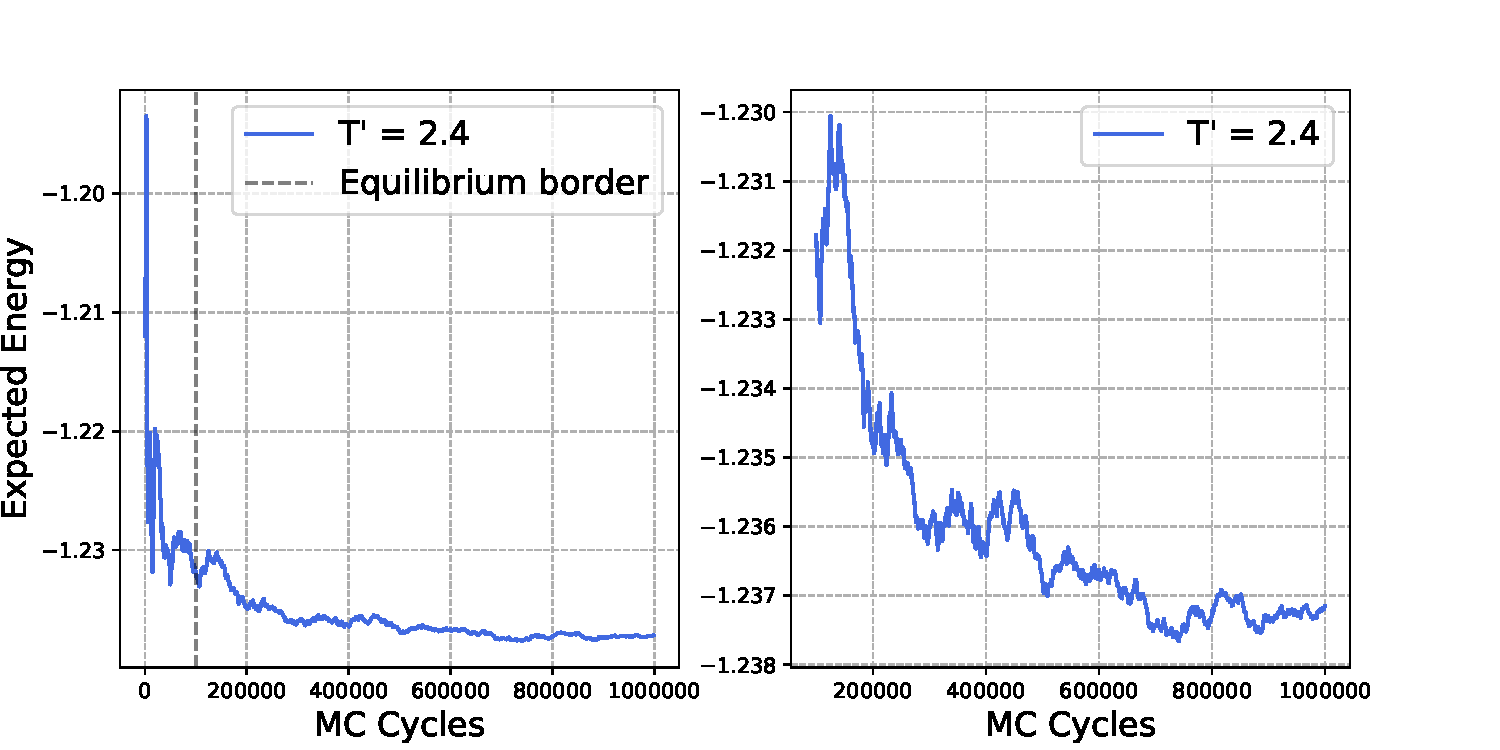
\includegraphics[width=1\textwidth]{figures/subEquilibriumE.pdf}
    \caption{Equilibrium estimate of the energy expectation value for a system with $T' = 2.4$ using the lazy method. The left subfigure shows where the equilibrium transition occurs. The right subfigure shows a close up of the post equilibrium state expectation values.}
    \label{fig: Equilibrium}
\end{figure}

\subsubsection{Accepted Configurations} Another interesting system property is the frequency of which the Metropolis condition accepts a move / state. By extracting the number of accepted states for the above discussed simulations we can plot them as functions of number of MC cycles. This is done in the scatter plot seen in figure \ref{fig: Accepted}.

\begin{figure}
    \centering
    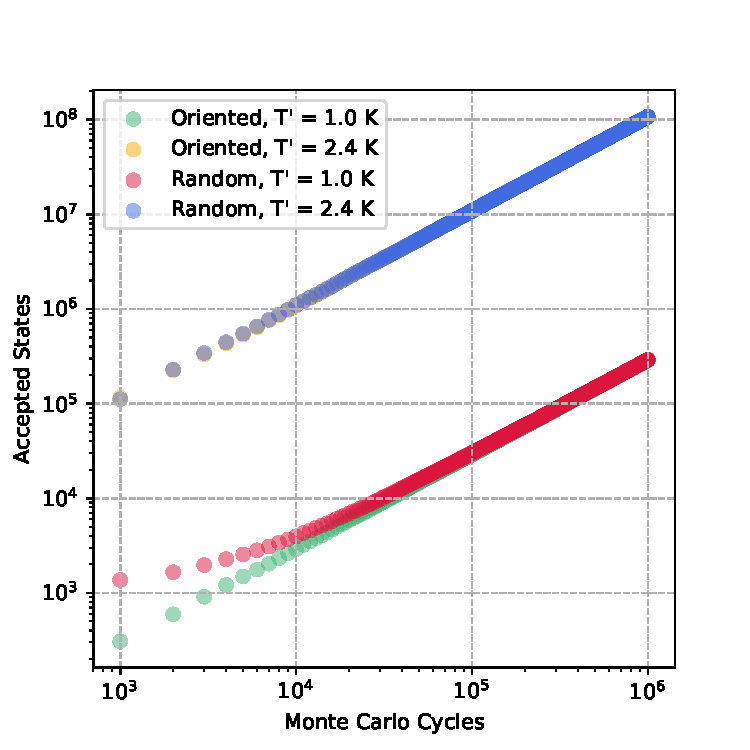
\includegraphics[width=0.78\textwidth]{figures/AcceptedStates.pdf}
    \caption{Number of accepted states as a function of MC cycles for 4 different $L = 20$ lattice simulations with oriented and random initial lattice configuration for temperatures $T' = 1$ and $T' = 2.4$.}
    \label{fig: Accepted}
\end{figure}

First of all, we note that the number of accepted states increases linearly with MC cycles for both $T' = 1$ and $T' = 2.4$. For $T' =2.4$ we see little to no difference between the number of accepted states for either configuration. The number of accepted states are much higher for $T' = 2.4$ compared to $T' = 1$ suggesting that the number of accepted states increase with the temperature of the system. This is the expected behaviour a higher temperature / energy means that the system can reach more states. Increasing the temperature of the system can therefore be viewed as "unlocking" more possible states.

For $T' = 1$ we see that the simulation with the random initial configuration results in more accepted states early on. This coincides with the previously mentioned statement that an ordered configuration better represents the true system. Since the oriented configuration is closer to equilibrium, it is has a lower probability to pass to Metropolis condition compared to the random configuration initially.


\begin{figure}
    \centering
    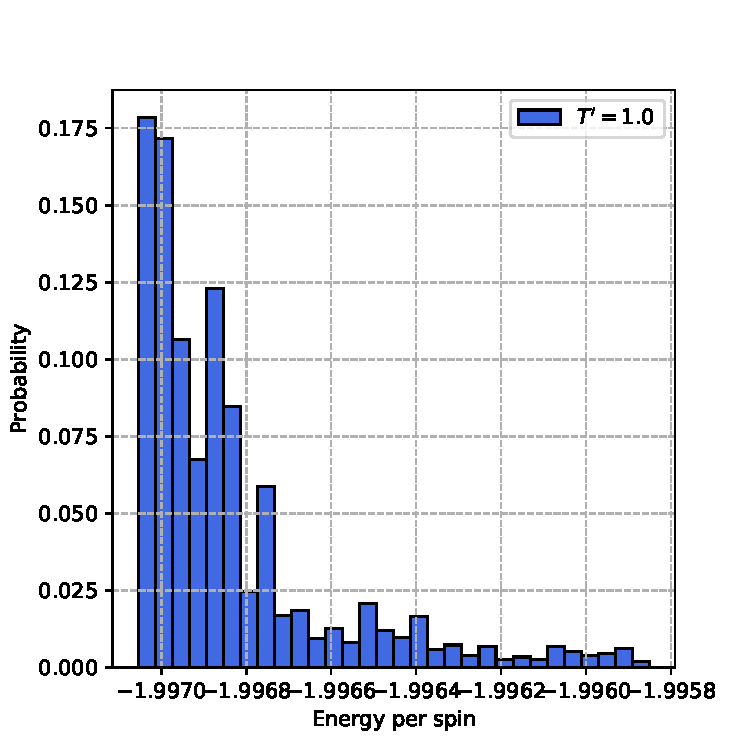
\includegraphics[width=0.78\textwidth]{figures/prob1.pdf}
    \caption{The probability distribution of the energy $P(E)$ for a $L = 20$ simulation with temperature $T' = 1$ and $10^5$ MC cycles.}
    \label{fig: prob1}
\end{figure}

\begin{figure}
    \centering
    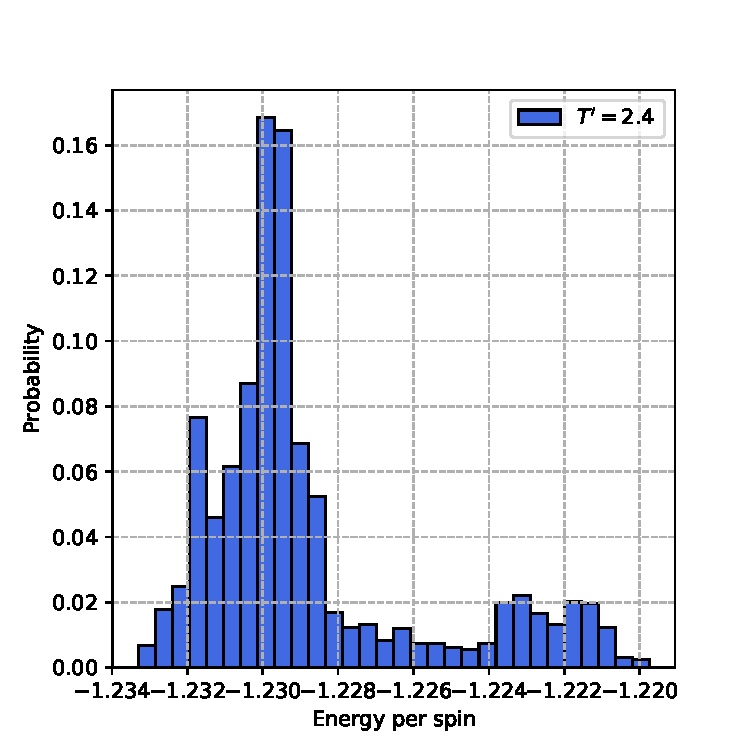
\includegraphics[width=0.78\textwidth]{figures/prob24.pdf}
    \caption{The probability distribution of the energy $P(E)$ for a $L = 20$ simulation with temperature $T' = 2.4$ and $10^5$ MC cycles.}
    \label{fig: prob24}
\end{figure}

\subsubsection{Probability Distribution} The final study of the $20 \times 20$ lattice will consider the probability distribution of the energy $P(E)$. We can look at how the energies are distributed in the above studied simulations by making a histogram of how often the different quantized energies occur. We have chosen to use a random initial configuration for the probability distribution. We have also used $10^5$ MC cycles where we have kept every computed expectation value to give a larger set of data. The results of the distribution can be seen in figures \ref{fig: prob1} and \ref{fig: prob24}.

The probability distribution for $T' = 1$ in figure \ref{fig: prob1} tells us that the energy which occurs most frequency is around $E \approx -1.997$ which matches the expectation value seen in the above studied figures. The same is true for the probability distribution for $T' = 2.4$ where $E \approx -1.231$. These values might differ slightly as the probability distributions here are done for $10^5$ MC cycles while the figure \ref{fig: 20x20 random <E> } has $10^6$. We can also study the respective energy variance for these simulations. We find that the variance for $T' = 1$ is $\sigma^2_E = 0.05165$ which corresponds to a standard deviation of $\sigma_E = 0.2252$. Similarly for the $T' = 2.4$ we find $\sigma^2_E = 7.8929$ and $\sigma_E = 2.8094$. These values correspond to the properties of the histograms. Comparing these values to standard deviations computed using the  \texttt{numpy.std} function we find that both standard deviations have nearly identical numerical values but numpy's estimate is of orders $10^3$ smaller than those we have calculated. For instance, $T' = 1$ numpy gives a standard deviation of $0.00023$ from numpy which better corresponds to the observed histogram features. The reason for this magnitude error is not understood on my part, but it might be a result of a scaling error somewhere in the calculations.

\subsection{Larger Systems $L \in [40,60,80,100]$}
We have now acquired a good intuition into the behaviour of the Ising model for the $20 \times 20$ lattice and will now move on to study the model for non static temperatures. We are interested in looking at how the expectation values behave close to the critical temperature, and will therefore compute them as functions of temperature rather than MC cycles. The temperature range of choice is 1000 temperatures $T' \in [2.0,2.4]$, giving us a $\Delta T' = 0.0004$. This is done in order to get a more continuous behaviour in the data. We will complete this study for lattice sizes of $L = 40$, $L = 60$, $L = 80$ and $L = 100$. 
\subsubsection{Expectation Values as function of Temperature}
The above conditions results in extensive computational times but are easily handled by the methods discussed previously in the methods section. The results of the simulation can be seen in figures \ref{fig: temp E}, \ref{fig: temp absM}, \ref{fig: temp CV} and \ref{fig: temp SUS}. These figures contain two subfigures. Subfigures (A) display the data points  for the various lattices sizes while the subfigures (B) show a best fit interpolation of these points. 

By studying the results of the average energy in figure \ref{fig: temp E} , we see that it behaves in a similar fashion independent of lattice size with the exception of some slight deviation after the critical temperature is crossed where the curve gets steeper with increasing lattice size. We also note that for low temperatures we observe some variation/noise in the expectation value.

In figure \ref{fig: temp absM} we see the absolute magnetization. The reason we plot the absolute value of the magnetization instead of just the magnetization is to avoid the possibility of the magnetization oscillating between negative and positive values below the critical temperature. This can occur after a given number of MC cycles where the net spin might be slightly positive but can still occasionally suddenly switch to negative value, as this is still a equally valid state. We observe that all lattices sizes behaves similarly for low temperatures. As the temperature increases, the magnetization starts to drop. The larger lattice sizes experience a sharper drop and end up with a lower final value before they flatten out. After the phase transition the net magnetization should be 0, which is the behaviour we want to observe. Since larger lattices are better approximation of true systems, we expect simulations with higher $L$'s to get closer to 0. We do observe a similar tendency where the the final magnetization is approaching 0 with increasing lattice size.

The specific heat can be studied in figure \ref{fig: temp CV}. We note the heat capacity develops shaper and sharper peaks with increasing lattice sizes which are centralized around the critical temperature. These peaks can be used to determine the system specific critical temperature. In subfigure (B) we have included stippled lines for each of the different lattice size which intersect both the maxima of the peaks and the temperature-axis. This intersection point is the critical temperature, and we find them to be $T_C(L=40)=2.285$, $T_C(L=60)=2.281$, $T_C(L=80)=2.278$ and $T_C(L=100)=2.273$. 

Similarly to the specific heat figure, the susceptibility seen in \ref{fig: temp SUS} also behaves by reaching increasingly sharper peaks for larger and larger lattice sizes. From the data points seen in subfigure (A) we see that this is a discontinuous process, where the susceptibility remains low before instantly jumping to the maximum value at the critical temperature. We have again created a best fit interpolation which allows us to study the peaks. Similarly to the specific heat, the intersection between the maximum values and the temperature axis gives us the critical temperatures. We find them to be $T_C(L=40)=2.270$, $T_C(L=60)=2.278$, $T_C(L=80)=2.282$ and $T_C(L=100)=2.283$. These critical temperatures are then averaged with the ones obtained from the specific heat and are tabulated in table \ref{tab: T_C}.

The observed noise for the low temperatures appear only for the large lattice simulations. This is likely a result of the initial configuration as they only appear in the low temperature range. From our analysis we know that an ordered lattice is a better approximation for the system at low temperatures. Another factor might be that the system has not reached equilibrium before we start computing expectation values.


\begin{table}[]
\caption{The critical temperatures for a given lattice size obtained by averaging the critical temperatures extracted from the specific heat and susceptibility results.}
\label{tab: T_C}
\begin{tabular}{|c|c|c|c|c|}
\hline
L:       & 40     & 60     & 80     & 100    \\ \hline
$T_C(L)$ & 2.2778 & 2.2796 & 2.2800 & 2.2782 \\ \hline
\end{tabular}
\end{table}

\begin{figure}
     \centering
     \subfloat[][Gathered data.]{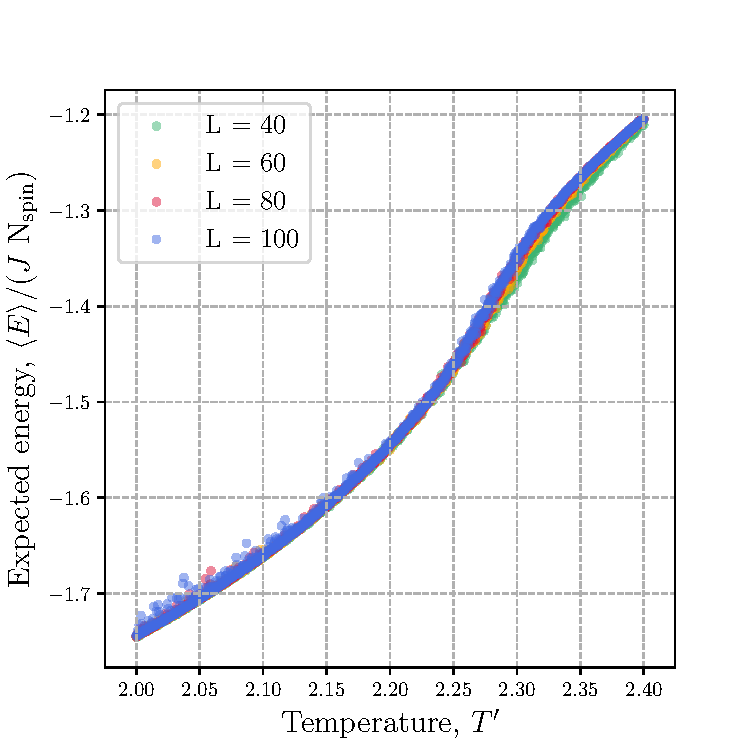
\includegraphics[width=0.5\textwidth]{figures/E.pdf}\label{fig: E}}
     \subfloat[][Best fit interpolation.]{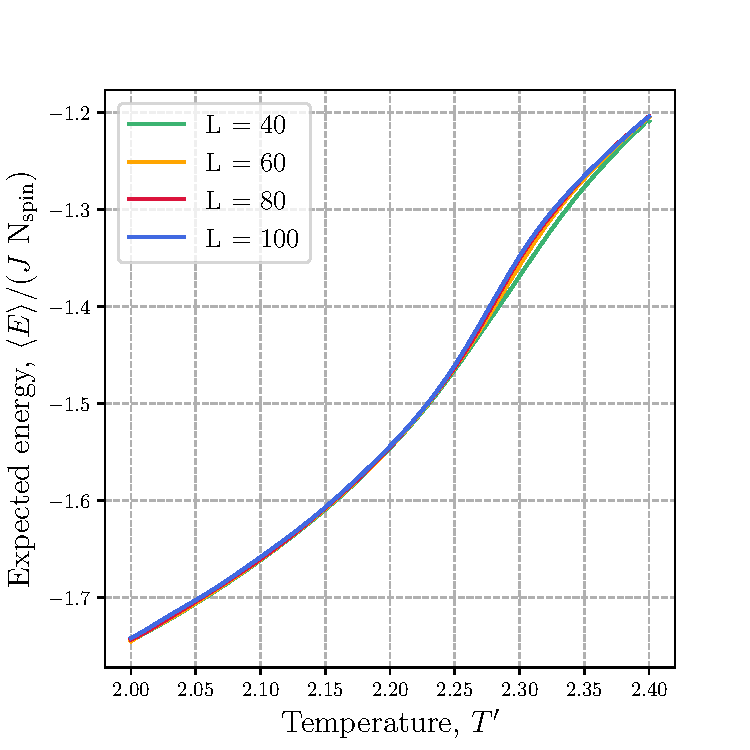
\includegraphics[width=0.5\textwidth]{figures/Ebest.pdf}\label{fig: E best}}
     \caption{The expectation value of the energy as a function of temperature for multiple sizes of $L$. Subfigure (A) displays the acquired data points while subfigure (B) displays a best fit interpolation curve to these data points.}
     \label{fig: temp E}
\end{figure}

\begin{figure}
     \centering
     \subfloat[][Gathered data.]{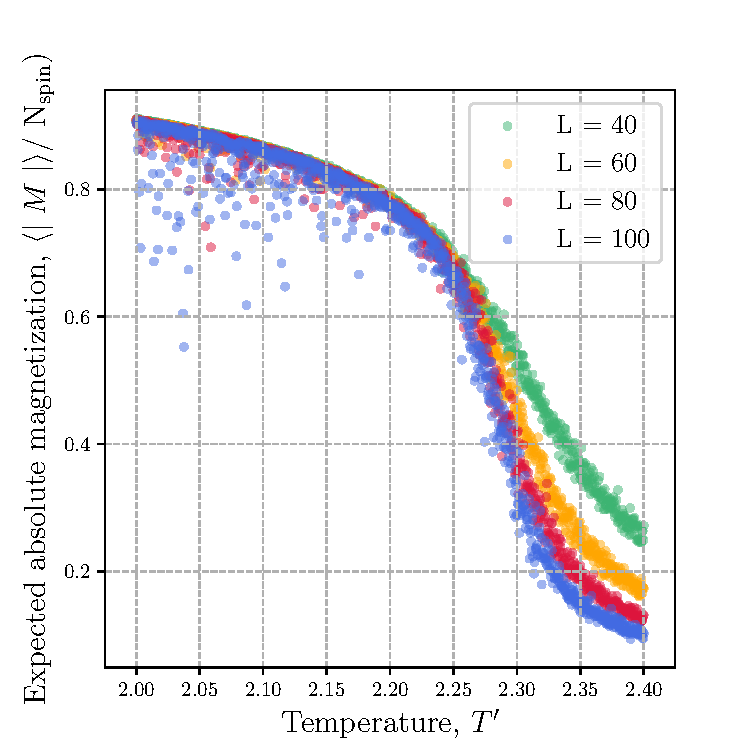
\includegraphics[width=0.5\textwidth]{figures/absM.pdf}\label{fig: E}}
     \subfloat[][Best fit interpolation.]{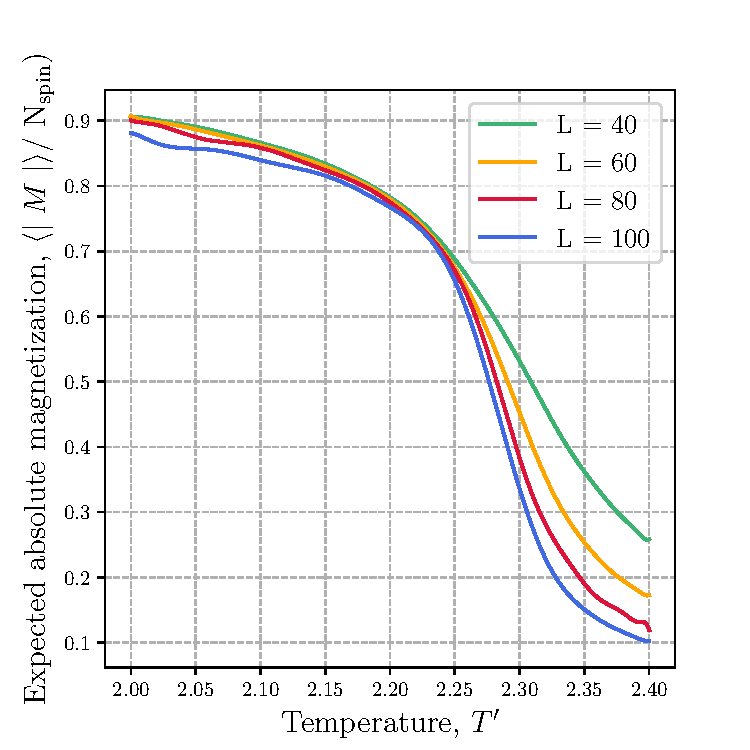
\includegraphics[width=0.5\textwidth]{figures/absMbest.pdf}\label{fig: E best}}
     \caption{The expectation value of the absolute magnetization as a function of temperature for multiple sizes of $L$. Subfigure (A) displays the acquired data points while subfigure (B) displays a best fit interpolation curve to these data points.}
     \label{fig: temp absM}
\end{figure}

\begin{figure}
     \centering
     \subfloat[][Gathered data.]{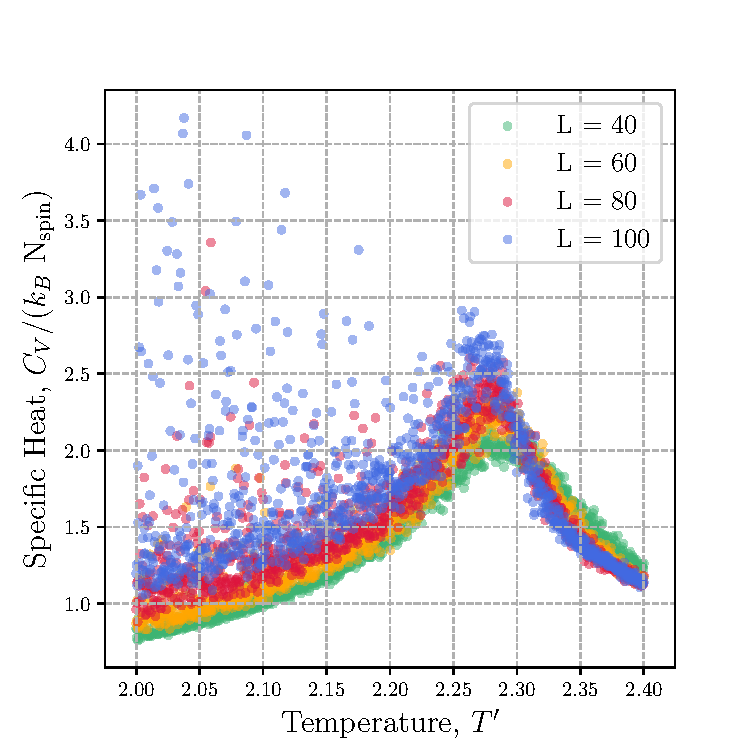
\includegraphics[width=0.5\textwidth]{figures/SH.pdf}\label{fig: E}}
     \subfloat[][Best fit interpolation.]{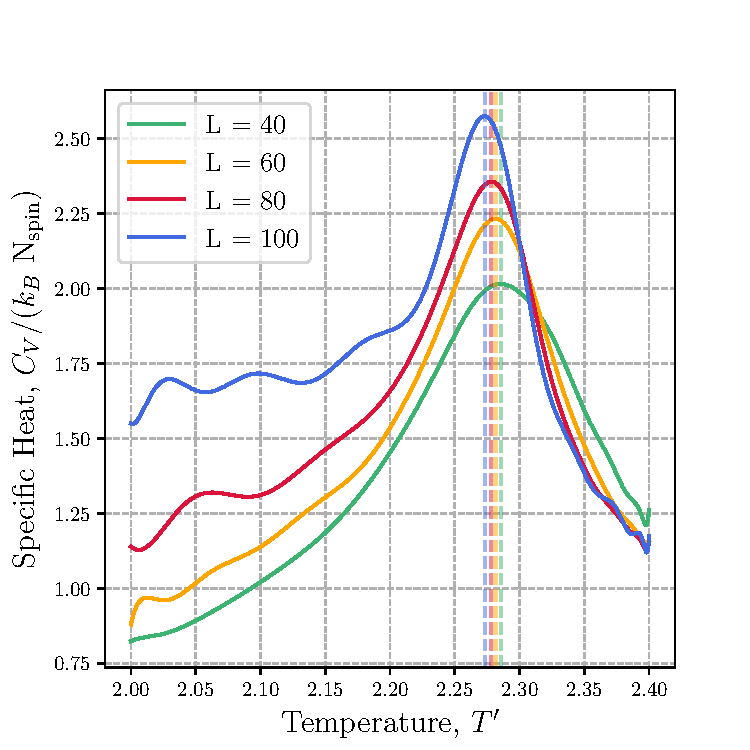
\includegraphics[width=0.5\textwidth]{figures/SHbest.pdf}\label{fig: E best}}
     \caption{The specific heat capacity as a function of temperature for multiple sizes of $L$. Subfigure (A) displays the aquired data points while subfigure (B) displays a best fit interpolation curve to these data points. The critical temperatures for each lattice size are $T_C(L=40)=2.285$, $T_C(L=60)=2.281$, $T_C(L=80)=2.278$ and $T_C(L=100)=2.273$}
     \label{fig: temp CV}
\end{figure}

\begin{figure}
     \centering
     \subfloat[][Gathered data.]{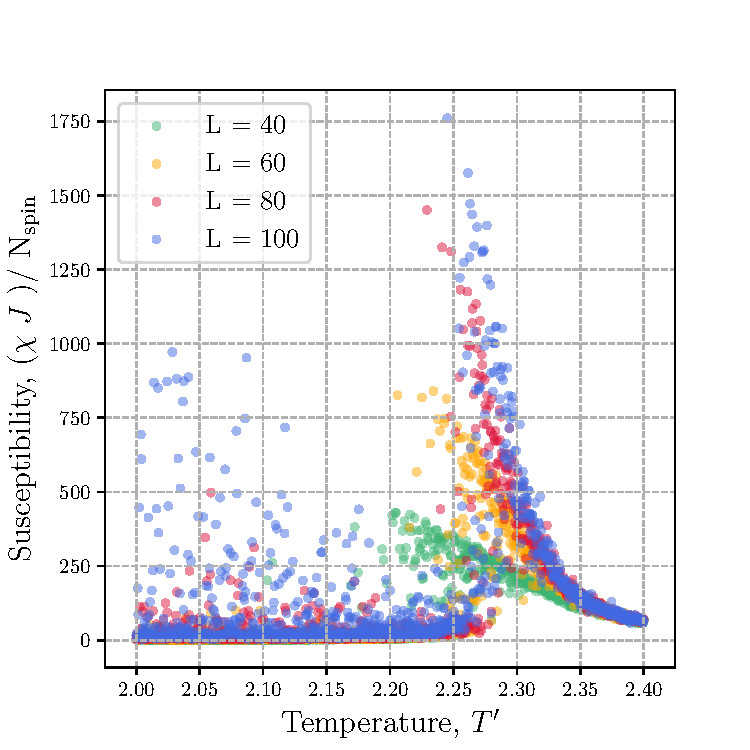
\includegraphics[width=0.5\textwidth]{figures/SUS.pdf}\label{fig: E}}
     \subfloat[][Best fit interpolation.]{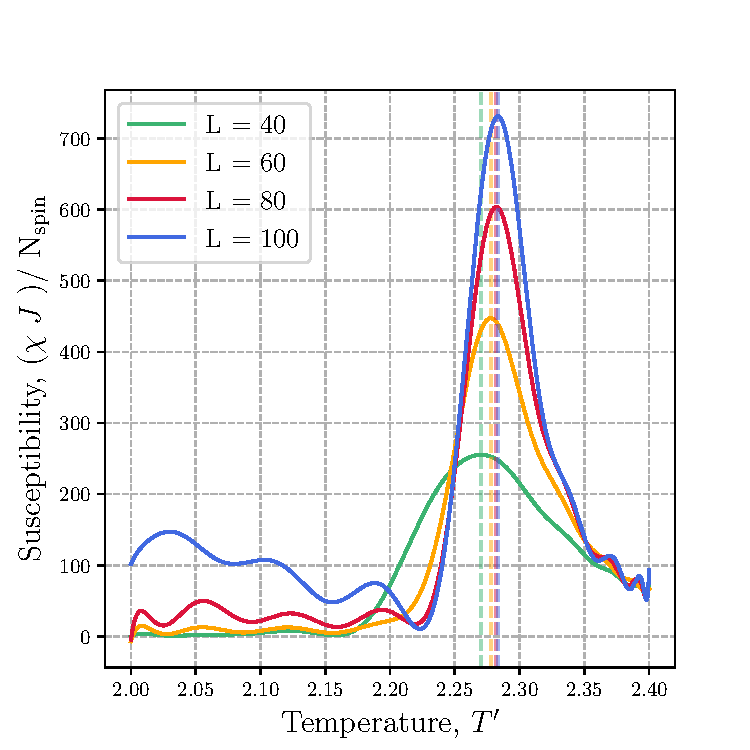
\includegraphics[width=0.5\textwidth]{figures/SUSbest.pdf}\label{fig: E best}}
     \caption{The susceptibility as a function of temperature for multiple sizes of $L$. Subfigure (A) displays the acquired data points while subfigure (B) displays a best fit interpolation curve to these data points. The critical temperatures for each lattice size are $T_C(L=40)=2.270$, $T_C(L=60)=2.278$, $T_C(L=80)=2.282$ and $T_C(L=100)=2.283$}
     \label{fig: temp SUS}
\end{figure}

\subsubsection{Estimating the Critical Temperature}

We are now able to compare our calculated critical temperatures with the exact results obtained by Lars Onsager. We can estimate the constant $a$ from equation \eqref{eq: a} by using the different critical temperatures in table \ref{tab: T_C} along with their respective lattice sizes. This is done for all unique lattice combinations. The computed values for $a$ are then averaged substituted into \eqref{eq: T_C} which gives us an estimate for the critical temperature at the thermodynamic limit $L \rightarrow \infty$. In order to get a better representative result, we solve this equation for all different lattice sizes and average the result. The result of this calculation leaves us with $T_C(L = \infty) = 2.2751\; J/k_B$. The obtained result is very close to the analytically derived critical temperature by Lars Onsagers and differ only by an order of $\sim 10^3$.

These calculations could be improved upon by adding simulations of larger lattices to the data set which would give us a better approximations to the results in the thermodynamic limit $L \rightarrow \infty$. Other areas of improvements are in the Monte Carlo method. These results are found using $10^5$ MC cycles per temperature step. Increasing this number in addition to dealing with the mentioned low temperature noise would give better best fit interpolations which would yield more accurate critical temperature estimates. The final method of finding $T_C(L=\infty)$ could also be switched up as many ways lead to Rome in this case. One could avoid calculating $a$ altogether by simply comparing two difference lattice sizes and solving those equations for $T_C(L=\infty)$.

The Metropolis algorithm is also not very efficient close to the critical temperature. Use of other methods such as the heat bath algorithm or the Wolff algorithm just to mention some would result in better near-critical temperature estimates. The Metropolis algorithm however is a simple and algorithm and is worth while in terms of its educational value.

\section{Conclusion}
The study of the two dimensional binary Ising model has lead to interesting and satisfactory results which compliment each other. We have worked our way through the $2\times 2$ lattice all the way up to the $100 \times 100$ lattice. We have been introduced to Monte Carlo methods and their random nature in addition to some insight into the functionality of RNGs. The results produced by our study are overall very good and are compatible with known results. 

There are still room for improvement as there always is, and some ideas for improvement has been discussed in the Results / Discussion section. Other ideas and future improvements might be to do more extensive calculations which higher orders of MC cycles. 

\nocite{*}
\bibliography{references}{}
\bibliographystyle{plain}
\end{document}
